\normaltrue
\correctionfalse

%\UPSTIidClasse{11} % 11 sup, 12 spé
%\newcommand{\UPSTIidClasse}{12}

\exer{Mouvement R  $\star$ \label{C2:08:02}}
\setcounter{question}{0}\UPSTIcompetence[2]{C2-08}
\UPSTIcompetence[2]{C2-09}
\index{Compétence C2-08}
\index{Compétence C2-09}
\index{Torseur cinétique}
\index{Torseur dynamique}
\index{Mécanisme à 1 rotation}
\ifcorrection
\else
\textbf{Pas de corrigé pour cet exercice.}
\fi

\ifprof
\else
Soit le mécanisme suivant. On a $\vect{AB}=R\vect{i_1}$ avec $R=\SI{20}{mm}$. 
On note $m_1$ la masse du solide 1, $B$ son centre d'inertie et $\inertie{B}{1}=\matinertie{A_1}{B_1}{B_1}{0}{0}{0}{\bas{1}}$.

\begin{center}
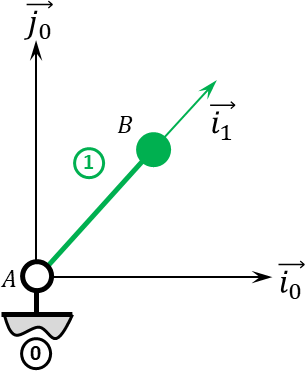
\includegraphics[width=\linewidth]{02_R_01}
\end{center}
\fi

\textbf{Méthode 1 -- Déplacement du torseur dynamique}

\question{Exprimer le torseur cinétique $\torseurci{1}{0}$ en~$B$.}
\ifprof
\else
\fi

\question{Exprimer le torseur dynamique $\torseurdyn{1}{0}$ en $B$ puis en $A$.}
\ifprof
\else
\fi

\textbf{Méthode 2 -- Calcul en $A$}


\question{Exprimer le torseur dynamique $\torseurdyn{1}{0}$ en $A$ (en utilisant une autre méthode que dans la question précédente).}
\ifprof
\else
\fi

\textbf{Masse ponctuelle}

On fait maintenant l'hypothèse que la masse est ponctuelle et concentrée en $B$.

\question{Exprimer le torseur cinétique $\torseurci{1}{0}$ en~$B$.}
\ifprof
\else
\fi

\question{Exprimer le torseur dynamique $\torseurdyn{1}{0}$ en $B$ puis en $A$.}
\ifprof
\else
\fi


\ifprof
\else
\begin{flushright}
\footnotesize{Corrigé  voir \ref{C2:08:02}.}
\end{flushright}%
\fi